%   %==========================================================================
%   %  Section
%   %==========================================================================
    \section{原子,分子の概念の導入}
        \begin{mycomment}
            最初に「化学」の分野で習う法則を確認するが,あくまでも量子力学を確認するためである.多
            くの量子力学の教科書は,「物質は多数の原理や分子の運動である」ということが当然のように記述
            されている.しかし,原子を肉眼で確認することは不可能である.どのように「物体は多数の原子や
            分子の集合である」ことを見出したのかについては書かれていないことが多い.

            実は,分子や原子の概念は「化学」の分野で最初に導入された.当然,分子・原子を観測することは
            できなかったのだが,化学反応という現象を説明するには,原子や分子という概念を導入する必要が
            あったのである.そこで,このノートでは分子や原子の導入のために,簡単な化学反応を最初に確
            認したいのである.

            なぜ,物質は小さな原子の集まりである,といわれるのだろうか.
            ここでは,その原子という概念の導入となる,
            いくつかの化学の法則を見ていくことにしよう.

            使用する教科書は,
                \begin{itemize}
                    \item 竹内 敬人 [著],
                            『化学の基本6法則』,岩波ジュニア新書,1982
                    \item 小川 岩雄 [著],
                            『原子と原子核』,共立出版,2008
                    \item Steven Weinberg [著],本間 三郎 [訳],
                            『(新版)電子と原子核の発見』,ちくま学芸文庫,2009
                    \item Isaac Asimov [著],玉虫 文一$\cdot$竹内 敬人 [訳]
                            『化学の歴史』,ちくま学術文庫,2010
                \end{itemize}
            である.
        \end{mycomment}

%       %======================================================================
%       %  Subsection
%       %======================================================================
        \subsection{定比例の法則}
            リヒター
                \footnote{
                    Jeremias Benjamin Richter (1762--1807,ドイツ),化学者
                },
            プルースト
                \footnote{
                    Joseph Louis Proust (1754--1826,フランス),化学者
                }
            は定比例の法則を発見する.

                \begin{myshadebox}{定比例の法則}
                    与えられた物質の成分元素の質量比は一定である.
                \end{myshadebox}

            水を例にとってこの法則を考えてみる
                \footnote{
                    気体の例を挙げるよりも,身近な水の例を挙げたほうがわかりやすいと思う.
                }.
            水は水素と酸素から構成されている.定比例の法則が意味するのは,水を構成する水素と酸
            素の質量比が一定だということである.もっと簡単にいえば,「水を構成する水素と酸素は
            いつでも同じ割合いなっている」ということである.具体的には,水を構成する水素と酸素
            の比は,水素:酸素 $=$ 1:8 である
                \footnote{
                    ここで注意すべきなのは,“水素が1つに対して酸素が8つということではない”
                     ということである.あくまでも質量比である.水素1[$\mathrm{g}$] に対して,
                     8[$\mathrm{g}$] の酸素が反応するということである.9[$\mathrm{g}$]の酸素が
                     存在しても,そこに水素が1[$\mathrm{g}$]しかない場合,この水素と酸素が反応
                     した後,1[$\mathrm{g}$]の酸素が残るのである.
                }.

%       %======================================================================
%       %  Subsection
%       %======================================================================
        \subsection{倍数比例の法則}
            ドルトン
                \footnote{
                    John Dalton(1766--1844,イギリス):原子説を強く唱えた科学者.ボイルやラヴォアジエ
                    らの実験事実に基づく理論構築を行った.
                }
            はこの \textbf{倍数比例の法則} を提唱し,物質の原子説を発表した.この理論により,原子説が有力になり,
            物質の変化を原子の観点から,考察されるようになった.
                \begin{myshadebox}{倍数比例の法則}
                    2種類の元素が2つ以上の化合物を形成するとき,一方の元素の一定量と化合する他方の
                    質量は互いに簡単な整数比になる.
                \end{myshadebox}

            同じ二つの種類の元素からなる化合物を,2種類考えてみよう.例えば,CO(一酸化炭素)と
            CO${}_{2}$にしよう.たしかに,COとCO${}_{2}$は,両方ともにC(炭素)とO(酸素)の二種類の元
            素から構成されている.
            例えば,炭素Cを一定量とすると,一酸化炭素と二酸化炭素のそれぞれに含まれる酸素の比は 1:2 である
                \footnote{
                    現在の化学記号は,すでに倍数比例の法則が反映されているため,
                    この法則を説明するのに化学記号を使って説明を行うと,
                    記号を見れば明らかではないか,と思われるかもしれない.
                }.

%       %======================================================================
%       %  Subsection
%       %======================================================================
        \subsection{ドルトンの原子説}
            物質を構成するものには基本的なものがある.この基本的の物質を“\textbf{元素}(element)”
            という.もう少し正確に元素を定義するならば,
                \begin{center}
                    “\textbf{元素}”とは「それ以上に単純な物質に分けられないもの」である.
                \end{center}
            と言える.「元素」に“ ”をつけたのは,現在は元素の定義として,この定義を用
            いていないからである.現在は,上の「それ以上に単純な物質に分けられないもの」で定義され
            る量は,\textbf{単体} とよばれている.

            ドルトンから始まる原子説は,単に化学現象を理論的に説明するために作られた,
            思考上の概念であった.原子の実在性は,この後,物理学者に再度疑われ
                \footnote{
                    力学史で有名なマッハは,原子説に対して批判的であったらしい.
                },
            さらなる実験がなされることになる.

%       %======================================================================
%       %  Subsection
%       %======================================================================
        \subsection{気体反応の法則,アヴォガドロの分子説}
            ゲイ・リュサック
                \footnote{
                    Joseph Louis Gay-Lussac(1778--1850, フランス):フランスの
                    化学者.
                }
            は,気体同士の反応に関する法則を発見した.
            \begin{myshadebox}{気体反応の法則}
                気体間が化学反応するとき,反応する気体の体積と生成する気体の体積の間には簡単な
                整数比が成立する.
            \end{myshadebox}

%   %==========================================================================
%   %  Section
%   %==========================================================================
    \section{原子模型}
            \begin{mycomment}
                \textbf{原子模型} とは 原子構造の模型のことをいう.
                化学の世界で,原子の存在が確かになってくると,その次の段階として,原子の構造に興味
                が湧くのは当然のことだろう.ここでは,原子の構造はどのようになっているかを考えた人
                の,いくつかの提案(構造の模型)を見ていくことにしよう.はじめに注意しておくと,これ
                らの模型は量子力学的に間違ったものである.しかし,量子力学を考慮しない範囲では有用
                な考え方であり,実際に物体をマクロで考えるときにはこの原子模型を用いて話をされるこ
                とが多い.
            \end{mycomment}

%       %======================================================================
%       %  Subsection
%       %======================================================================
        \subsection{電子の発見}
            電子の発見は,マクスウェルによって電磁気学が確立された後のことである.電磁気学の部分で保留
            にしていた電子の発見について,ここで確認しておこう.原子は電気的に中性である.「電気的
            に中性」というのは正の電荷も負の電荷ももたないということである.原子がその内部に電子を
            含むので,この電子のもつ負の電荷とちょうど相殺するような正電荷を原子はもっていることに
            なる
                \footnote{
                    「物質を構成する最小の単位は原子である」という仮定をしていることを前提とした主
                    張である.
                }.
            この正電荷が陽子である.原子がどのような形で陽子をもっているかについては,2通り考えら
            れる.1つは陽子と電子が混在しているものである.この構造はトムソンによって提案されたの
            で \textbf{トムソンの原子模型} とよばれる.もう一つは,陽子の周りを電子が回転していると
            いうものである.この構造は,日本人の長岡半太郎によって提唱されたものである.この長岡の
            原子模型では,電子は平面上の楕円軌道を描くとされる.土星のような模型である.土星の輪が
            電子の描く軌道に相当する.この模型の拡張とのいうべきものが,ラザフォード
                \footnote{
                    Ernest Rutherford(1871--1937, イギリス):原子核の発見(実験),$\alpha$線と
                    $\beta$線の発見などで有名.放射線に $\gamma$線という名前を与えたのもこの人.
                    元素崩壊と放射線の業績(化学)を理由に,ノーベル化学賞を受賞している.
                }
            によって提案され
            た.\textbf{ラザフォードの原子模型} では,電子は1つの平面における単なる楕円軌道ではなく
            ,楕円軌道が刻々と変化するというものである.ラザフォードらの実験によれば,
            原子の形はラザフォード模型であることが確認される.しかし,この原子模型には欠
            点がある.後で確認することだが,陽子の周りを電子が回転すると電磁波が生じる.この電磁波
            は電子のもつエネルギーを外部に放射してしまう.このため,原子の速度が減少し,電子が陽子
            の周りを回転するために必要な速度が保てなくなる.すなわち,電子が陽子とくっついて,原子
            がつぶれてしまうのである.このラザフォード模型の欠点は,\textbf{量子力学} という新しい物
            理学の分野を待たなければ解決することができない.

            話が前後するが,電子のもつ電気量の測定は「ミリカンの油滴実験」が有名である.もちろん,
            この実験の原理はマクスウェル方程式によって説明される.

%       %==========================================================================================
%       %  SubSection
%       %==========================================================================================
        \subsection{ラザフォードの原子模型(原子核の発見)}
            原子構造は,正電荷を持った原子核の周りに,負電荷を持った電子が周っている模型が
            知られている.こうした今日知られている原子模型は,ラザフォードによるものである.
            ラザフォードは,原子構造を模索している中の実験で,奇妙な結果(\textbf{ラザフォード散乱})を得て,
            この結果から,現在知られている原子模型作り上げた.

            ラザフォードは,金属の薄膜に$\alpha$線を照射して,その透過具合や散乱の程度を調べる
            実験を行った.その結果は,ある割合で,$\alpha$線が透過せずに跳ね返ってくること
            が判明した.
                \begin{figure}[hbt]
                    \begin{center}
                        \includegraphics[keepaspectratio, width=4.6cm,height=2.95cm,clip]{RutherfordScattring.pdf}
                        \caption{ラザフォード散乱}
                        \label{fig:RutherfordScattring}
                    \end{center}
                \end{figure}

            その結果から,原子の構造は中心に正電荷をもった粒子があり,
            その正電荷の周囲に電子が存在する,という構造を導き出した
                \footnote{
                    (参考)新版 電子と原子核の発見,S.ワインバーグ [著],本間三郎 [訳],ちくま文芸文庫:
                     特に,第4章に原子核に関する実験について詳しく書かれている.
                     この本には,トムソンの陰極線に関する実験や,ミリカンの電子に関する実験なども丁寧に
                     書かれている.
                }.
            電磁気学とニュートン力学に基づいて発案されたこの原子模型は,現在の量子力学では
            否定されてしまう.しかし,化学を考える場合や電子回路と考える場合などは,このモデルで
            十分であることが多い.
                \begin{figure}[hbt]
                    \begin{center}
                        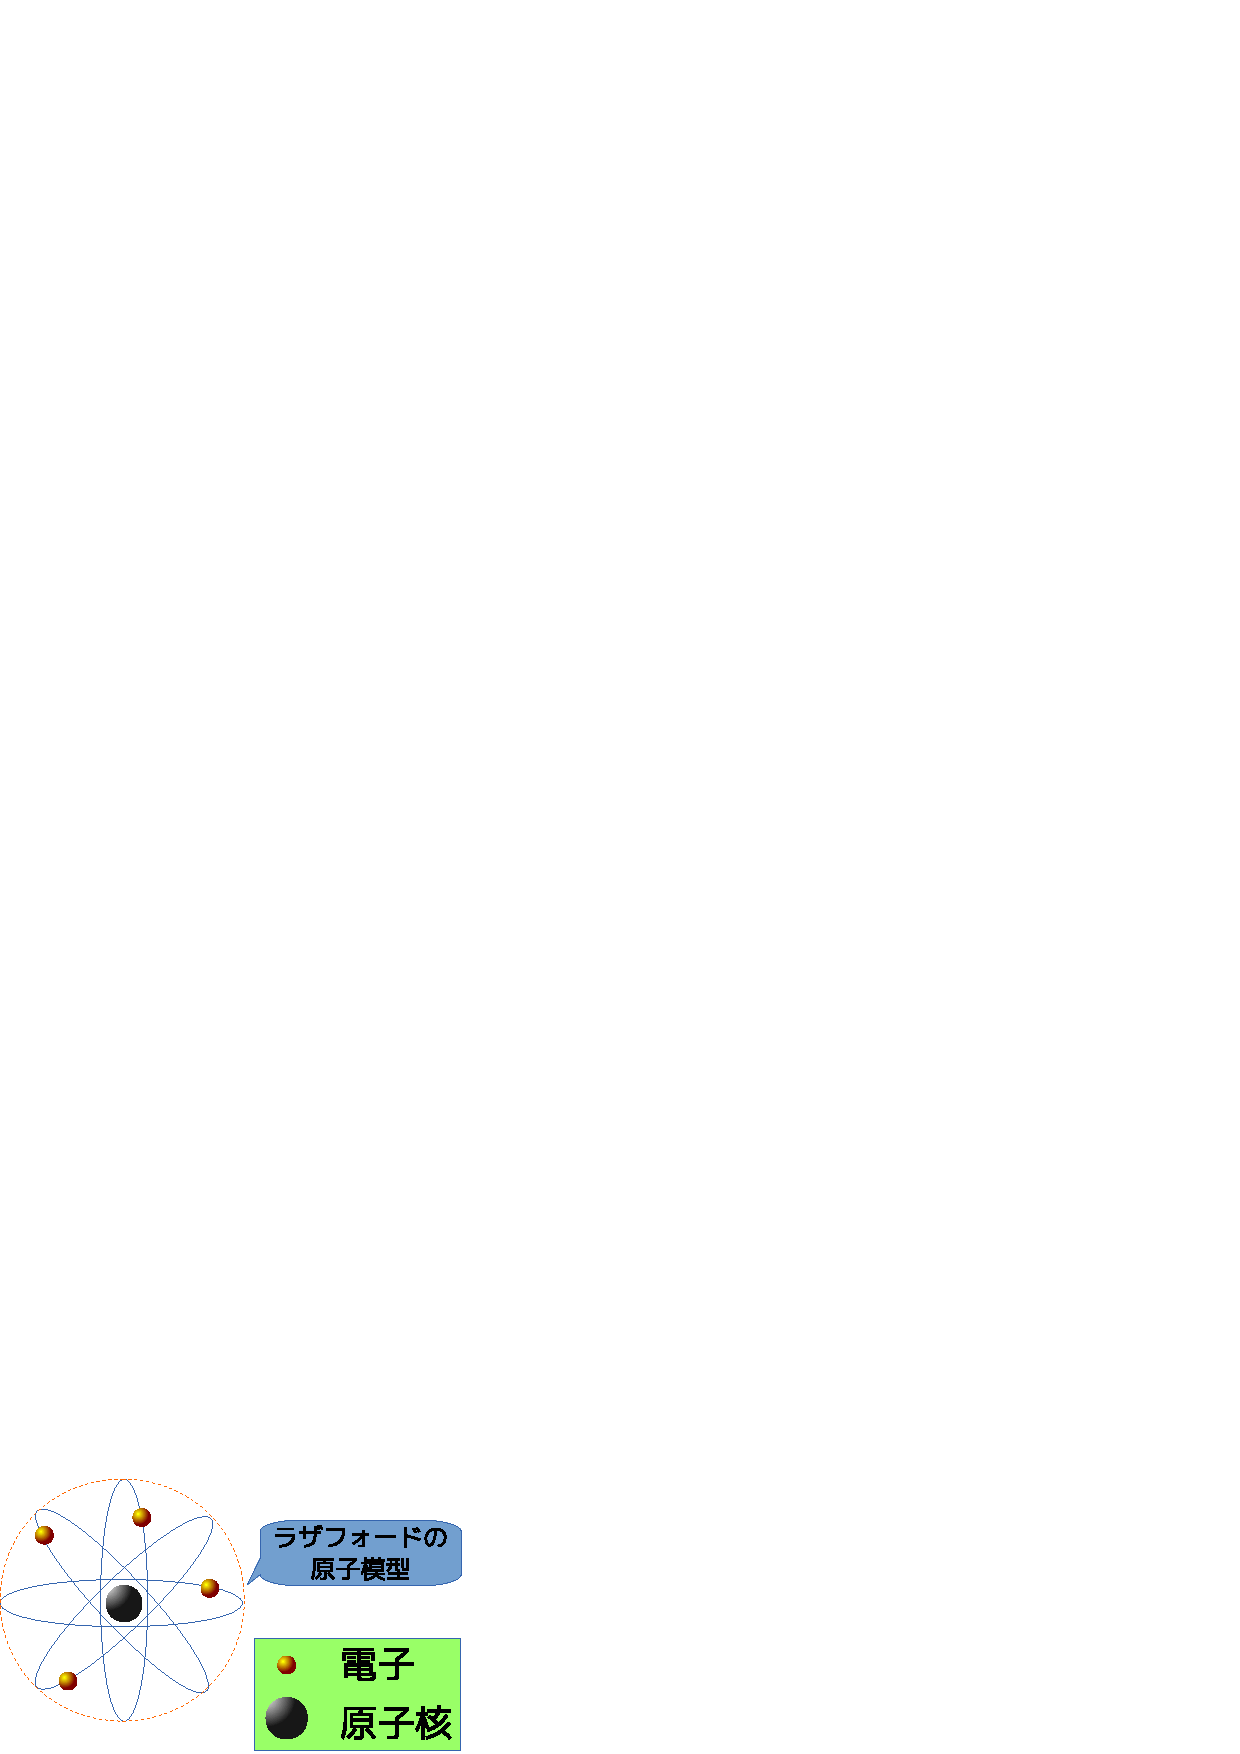
\includegraphics[keepaspectratio, width=4.0cm,height=2.56cm,clip]{RutherfordAtomModel.pdf}
                        \caption{ラザフォードの原子模型}
                        \label{fig:RutherfordAtomModel}
                    \end{center}
                \end{figure}

        \begin{memo}{トムソンの原子模型}
            ラザフォードによる原子構造の発見よりも前に,トムソンは \textbf{陰極線} という
            現象を発見している.陰極線とは,真空中に2つの電極を用意し,この電極間に高電圧をかけると,
            負電極から正電極に向かって何らかの粒子が飛ぶ現象である.陰極線という名前は,
            その性質からトムソン自身によって与えられた.実は,この陰極線は後に電子であることが判明する.

            電子は,負極から正極へと走ることから,負電荷であることがわかる.多くの物質は電気的に
            中性であることから,電子の負電荷はどこかで中和されているはずである.要するに,どこかに
            正電荷をもつ部分があるということだ.

            トムソンの時代には,物質は原子から構成されているという
            ことは,仮説でしかなかったが,トムソンはこの仮説を支持していた.そこで,トムソンは
            原子の模型として,正電荷をもつ領域内に電子がその正電荷を中和するように存在するという,
            原子模型を提唱した.この原子模型を \textbf{トムソンの原子模型} という.
                \begin{figure}[hbt]
                    \begin{center}
                        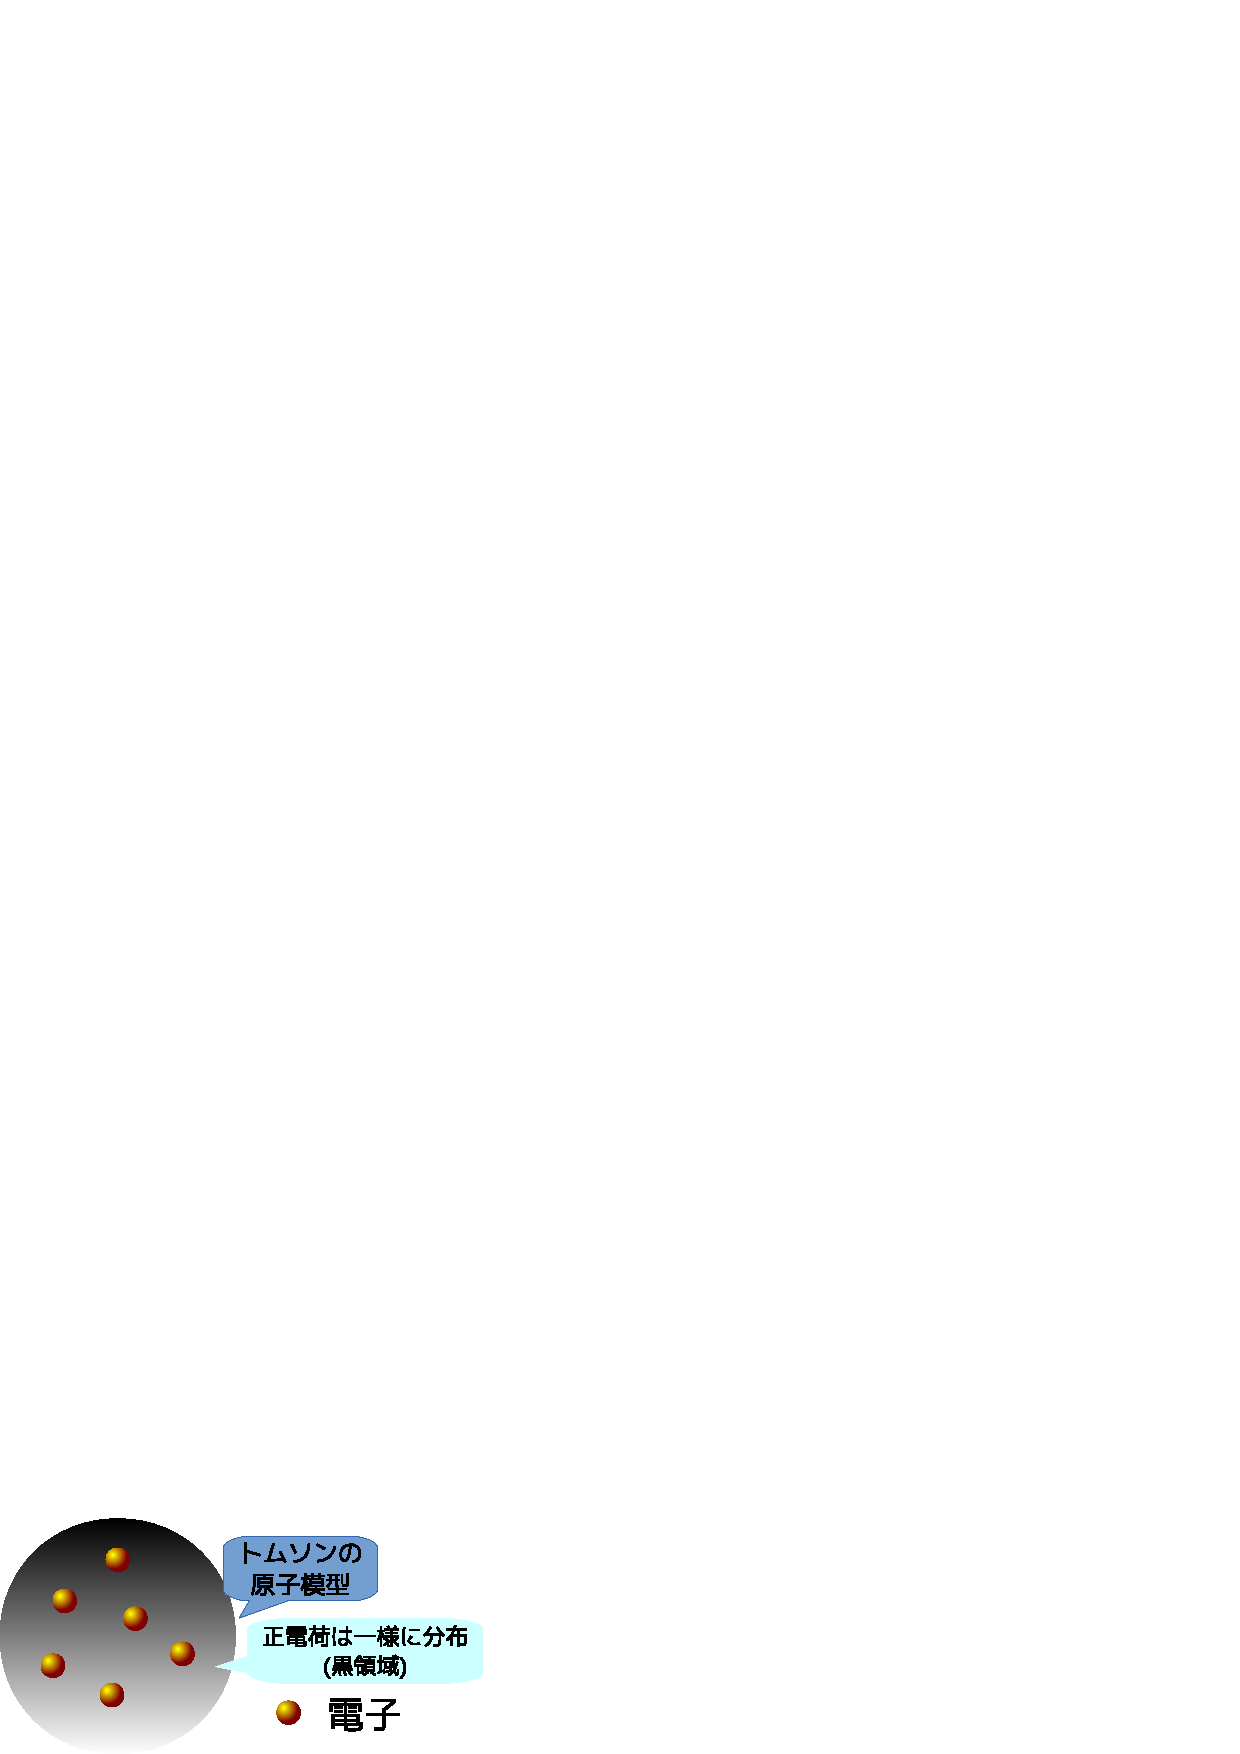
\includegraphics[keepaspectratio, width=5.05cm,height=2.5cm,clip]{TomsonAtomModel.pdf}
                        \caption{トムソンの原子模型}
                        \label{fig:TomsonAtomModel}
                    \end{center}
                \end{figure}
        \end{memo}

        \begin{memo}{長岡の原子模型}
            日本の物理学者に,長岡半太郎
                \footnote{
                    長岡半太郎(1865--1950, 日本):東京大学出身の,日本の物理学の先駆者的存在.土星型の
                    原子模型を提唱したことで有名.後世の教育にも努力された.
                }
            という人物がいる.長岡も原子模型を
            提唱していたらしく,Webサイトを検索するといくつかヒットする.
            電気学会の電磁気学の教科書にも紹介されている.長岡が提唱した
            原子模型は,ラザフォードの原子模型のを2次元にしたようなもので,
            よく化学の教科書に描かれているような元素の図がそのイメージに一致する.
                \begin{figure}[hbt]
                    \begin{center}
                        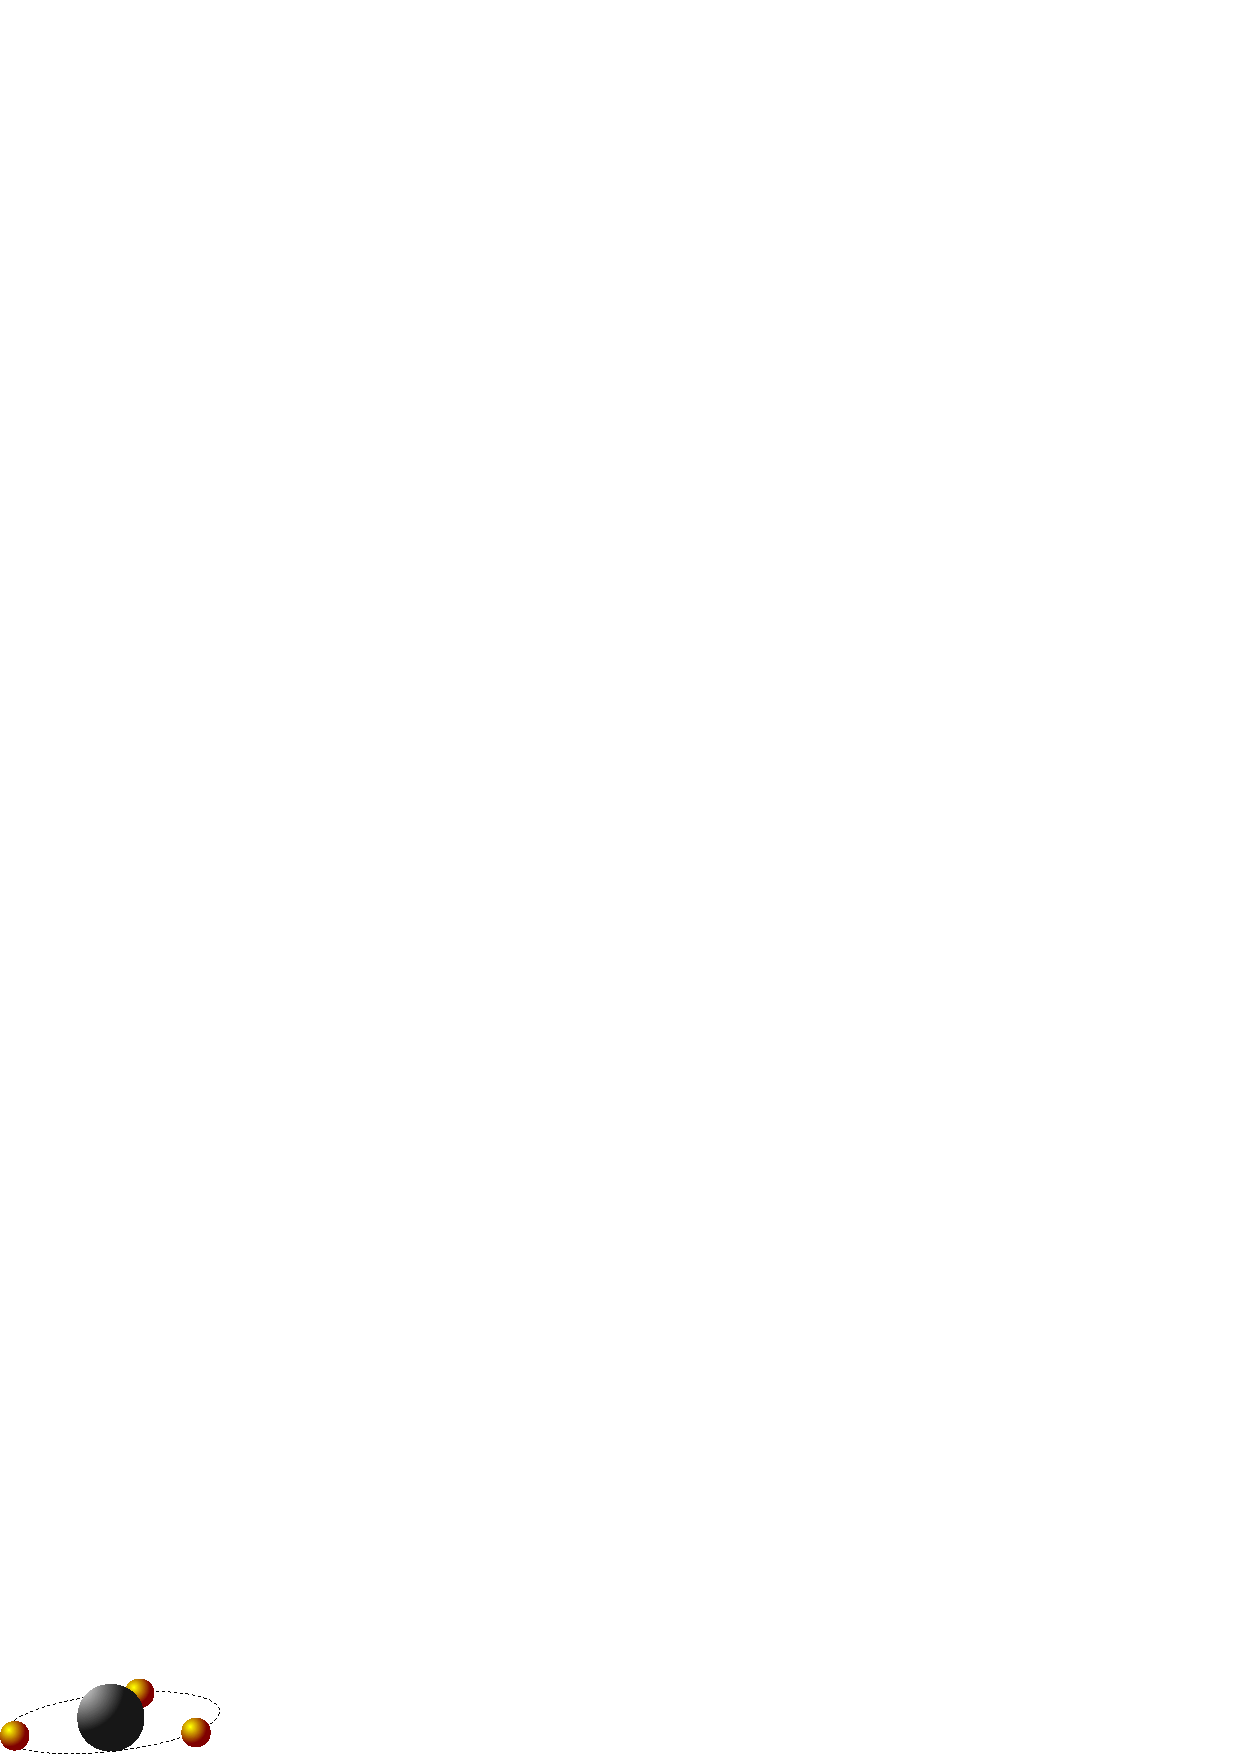
\includegraphics[keepaspectratio, width=3.8cm,height=1.3cm,clip]{NagaokaAtomModel.pdf}
                        \caption{長岡の原子模型}
                        \label{fig:NagaokaAtomModel}
                    \end{center}
                \end{figure}
        \end{memo}


        \begin{memo}{原子は本当に存在するのか}
            「原子」という概念は化学,つまり,物質の性質やその反応を理解するために導入されたもので
            ある.この「原子」という概念を導入することで,が矛盾なくしかも説明がスマートに行えるよ
            うになった.「原子」という概念を導入すれば,確かに,理論を綺麗に組み立てられることは確
            かであるが,実際に,「原子」そのものを見て,その存在を確認したわけではない.では,「原
            子」は,あくまでも理論を組み立てる上で導入する,“仮想”のもので,実際には存在しないも
            のなのだろうか.確かに,肉眼で
                \footnote{
                    あるいは,顕微鏡などで拡大して.
                }
            確認するまで,その存在を認めないと考えるならば,「原子」はただの仮想のものにすぎない.
            そうなると,現実には「原子」は存在せず,何かそれに変わるようなものがあると考えて,それ
            は今の人間には「原子」としてしか認識できないと考えることになるだろう.確かにそうかもし
            れない.この考えを完全に否定することはできない.

            しかし,科学を考える上で,このような考えは余り好ましくないと思う.科学の理論を支え
            る基板---つまり法則は,あくまでも“仮説”である.となれば,「原子」の存在を疑うことは
            ,法則を疑うことにつながる.科学は実験で得た結果に基づいて,推論し理論を組み立てていく
            作業である.それが,絶対に現実の世界と一致している必要はないのである.例えば,ニュートン力
            学は,アインシュタインによって,修正を加えられている.それまで,ニュートン力学はどのよう
            な場合でも
            成立すると考えられてきたと思うが,現実は違っていた
                \footnote{
                    ニュートン力学が仮定から完全に間違っていたわけではなかった.アインシュタインは,
                    考察対象と
                    なる系の速度が光速 $c$ に比べて,とても遅いことを暗黙の内に仮定していることを
                    指摘しただけである.そして,その修正とは,光速 $c$ に近い速度で運動する系でも
                    ,理論が矛盾なく成立するように拡張したものである.理論が全く書き換えられたわけ
                    ではない.理論には暗黙の内に仮定しているものがあるが,その暗黙の仮定は理論成立
                    時には気付けない.しかし,後に科学が発展して,“暗黙の内の仮定”に気付いたので
                    あれば,その都度,理論に修正を加えていけばよいのだ.
                }.
            ニュートン力学の修正のきっかけは,思考の範囲が広がったことと,実験の技術が向上したことに伴
            って,新しい実験結果を得ることができたからである.

            科学の理論とは,実験結果から推測される仮定に基づいて,構築されるものである.数学との違
            いをはっきりと意識させられるところである.

            このようなことから,原子の存在を,肉眼で観測できないからといって,疑う事は避けないとい
            けない.「原子」の存在を仮定して,現象の説明がスマートにできるのであれば,科学的に,“
            そこには「原子」がある”と主張されるのである.そしてこのとき,「原子」は科学的に実在す
            るのである.理論と実験結果の矛盾を見つけるまでは,「原子」の存在を仮定して話を進めてい
            くべきだ.
        \end{memo}


%           %==================================================================
%           %  Subsubsection
%           %========================s==========================================
%            \subsubsection{}

%   %==========================================================================
%   %  Section
%   %==========================================================================
    \section{原子核の構造}
%       %==========================================================================================
%       %  SubSection
%       %==========================================================================================
        \subsection{ウランの発見}
            クラプロート
                \footnote{
                    Martin Heinrich Klaproth(1743--1817, ドイツ):
                    化学者,薬剤師として活躍.
                    ウラン(酸化ウラン)の発見者として有名.
                }
            により,ウラン
                \footnote{
                    Uran,もしくは,Uranium
                }
            を発見する.

            クラプロートは,薬剤師としてドイツ各地で活躍していたが,
            薬学による治療では満足できず,化学的な手段に手を広げようとし,
            銀の発掘現場にて新たな鉱物が発見されたという情報聞をきつけ,
            閃ウラン鉱より,酸化ウランを取り出し発見した.
            「ウラン」の命名由来は,1781年にイギリスの天文学者ハーシェル
                \footnote{
                    Sir Frederick William Herschel(1738--1822, イギリス):
                    ドイツ生まれ.イギリスにわたり,音楽家として活躍する.
                    天文学にも興味を持ち,自身の手により望遠鏡を作成している.
                    その後,天王星を発見し,天文学の研究に専念する.

                    ドイツ語名ではFriedrich Wilhelm Herschelであったが,
                    イギリスに渡った後(1757年),Frederick William Herschelと名乗るように
                    なった.
                }
            が新しい惑星を発見し,「Uranus(ウーラノス,天王星)」を名づけたことを受け,
            これを讃えたことによる.

%       %==========================================================================================
%       %  SubSection
%       %==========================================================================================
        \subsection{X線の発見}
            レントゲン
                \footnote{
                    Wilhelm Conrad R\"{o}ntgen(1845--1923, ドイツ):
                    1901年に,第1回ノーベル物理学賞を受賞.受賞理由は
                    ,もちろん,X線の発見(1895年)による.1888年に,
                    マクスウェルが提唱した変位電流の存在を,
                    実験的に確かめている.
                }
            は(偶然的に)X線を発見した.

            放電管(クルックス管
                \footnote{
                    クルックス管:
                    Sir William Crookes(1832--1919, イギリスの物理学者,化学者)
                    による発明品.
                    トムソンの電子発見の説明でよく出てくる,真空管のこと.
                }
            )による放射現象の研究の中,
            感光処理を施した一枚の紙が発光していることに気づき,
            その原因を突き止めた結果,放電管から生じる目に見えない光線が
            放射されているがわかった.この光線が \textbf{X線} と呼ばれるものである
                \footnote{
                    \textbf{レントゲン線} とも呼ばれる.
                }.

%       %==========================================================================================
%       %  SubSection
%       %==========================================================================================
        \subsection{ウランから生じる放射線の発見}
            ベクレル
                \footnote{
                    Antoine Henri Becquerel(1852--1908, フランス):
                    物理学者.1903年に,放射線の発見により,ノーベル物理学賞
                    を受賞している.
                }
            は,ウランによる蛍光作用の研究の中,ウランから目に見えない放射が
            生じていることを発見した.(ポアンカレ
                \footnote{
                    Jules-Henri Poincar\'{e}(1854--1912, フランス):
                    数学者.アインシュタインの特殊相対性理論の先駆けとなる考察
                    (光速不変の原理など)や,ポアンカレ予想などで,その名が有名
                    である.とにかくものすごい数学者.
                }
            による示唆で,ウランの発光作用とX線との関連の研究を促されたらしい.)


%       %==========================================================================================
%       %  SubSection
%       %==========================================================================================
        \subsection{$\alpha$ 線と$\beta$ 線,$\gamma$ 線の発見}
        ラザフォードが $\alpha$ 線と$\beta$ 線を発見する.
        ピエール$\cdot$キュリーが $\gamma$ 線を発見する.
